% flashcards-title: Open number line showing an addition as two rightward jumps
% flashcards-desc: A horizontal number line with a dot on a mark labeled 34. A long curved arrow labeled plus 20 jumps right from 34 to a mark labeled 54, and a shorter curved arrow labeled plus 3 jumps right from 54 to a mark labeled with a question mark.
\documentclass[tikz]{standalone}
\usetikzlibrary{arrows.meta,patterns}

\definecolor{qraNavy}{HTML}{17324D}
\definecolor{qraBlue}{HTML}{2B6CB0}
\definecolor{qraGold}{HTML}{B7791F}
\definecolor{qraPale}{HTML}{EAF2F8}
\definecolor{qraGray}{HTML}{5C6773}

\tikzset{
  qra axis/.style={draw=qraNavy, line width=1.2pt},
  qra tick/.style={draw=qraNavy, line width=1pt},
  qra guide/.style={draw=qraGray, densely dashed, line width=0.8pt},
  qra counter/.style={circle, draw=qraNavy, fill=qraPale, line width=0.9pt, minimum size=7mm, inner sep=0pt},
  qra label/.style={font=\sffamily\bfseries, text=qraNavy},
  qra small label/.style={font=\sffamily, text=qraNavy},
}

\begin{document}
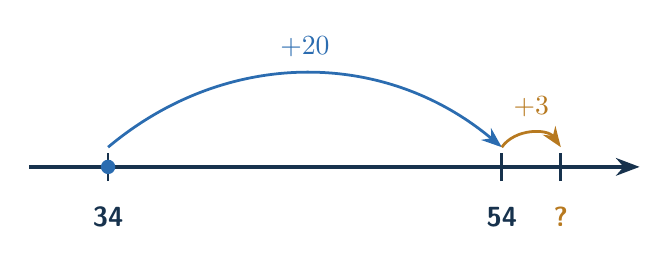
\begin{tikzpicture}[x=0.25cm]
  % Base line: 20 units span 5cm, 3 units span 0.75cm (honest proportion)
  \draw[qra axis, -{Stealth[length=3mm]}] (30,0) -- (61,0);

  % Ticks
  \foreach \x in {34,54,57} {
    \draw[qra tick] (\x,-0.18) -- (\x,0.18);
  }

  % Labels
  \node[qra label, below=6pt] at (34,-0.18) {34};
  \node[qra label, below=6pt] at (54,-0.18) {54};
  \node[qra label, text=qraGold, below=6pt] at (57,-0.18) {?};

  % Start dot
  \fill[qraBlue] (34,0) circle (2.6pt);

  % Jumps
  \draw[qra tick, draw=qraBlue, -{Stealth[length=2.6mm]}]
    (34,0.25) to[bend left=40] node[qra small label, above=2pt, text=qraBlue] {$+20$} (54,0.25);
  \draw[qra tick, draw=qraGold, -{Stealth[length=2.6mm]}]
    (54,0.25) to[bend left=55] node[qra small label, above=2pt, text=qraGold] {$+3$} (57,0.25);
\end{tikzpicture}
\end{document}
